\documentclass[aspectratio=169,11pt]{beamer}

% ================================================================
% "TABIIY TILNI QAYTA ISHLASH" KURSI
% MA'RUZA 9 --- Matn generatsiya va ikki tomonlama RNN
%              (d09_matn_generatsiya.tex)
% Arxetiplar: [A][B][C][D][E] + 4 tsikl [F][G][H][I][J][K][L] +
%             [M][N][O][P][Q][R] + ilova [S]
% Rendered slayd soni: ~45 (3-haftaning birinchi ma'ruzasi; L1-L8 chuqurligi)
% Qulflangan [I2]: temperature softmax T=1 p(nlp)=0.665, T=0.5 p(nlp)=0.867
%   --- P9 (Day 10) birinchi assert manbayi (course_map hand_example).
% ================================================================

% ================================================================
% RANGLAR  (asl fayldan o'zgarishsiz)
% ================================================================
\definecolor{cnublue}{rgb}{0.07,0.14,0.62}
\definecolor{cnubluelight}{rgb}{0.18,0.30,0.72}
\definecolor{cnubluebg}{rgb}{0.90,0.92,0.97}
\definecolor{deepblue}{rgb}{0.07,0.14,0.62}
\definecolor{deepred}{rgb}{0.60,0.00,0.00}
\definecolor{deepgreen}{rgb}{0.00,0.45,0.00}
\definecolor{halfgray}{gray}{0.55}

% ================================================================
% BEAMER MAVZU --- Boadilla + maxsus footer  (asl fayldan o'zgarishsiz)
% ================================================================
\usetheme{Boadilla}

\setbeamercolor{structure}{fg=cnublue}
\setbeamercolor{frametitle}{bg=cnublue,fg=white}
\setbeamercolor{title}{bg=cnublue,fg=white}
\setbeamercolor{block title}{bg=cnublue,fg=white}
\setbeamercolor{block body}{bg=cnubluebg,fg=black}
\setbeamercolor{alerted text}{fg=deepred}
\setbeamercolor{author in head/foot}{bg=cnubluelight,fg=white}
\setbeamercolor{section in head/foot}{bg=cnublue,fg=white}
\setbeamercolor{page number in head/foot}{bg=cnubluelight,fg=white}

\setbeamertemplate{mini frame}{}
\setbeamertemplate{mini frame in current section}{}
\setbeamertemplate{mini frame in current subsection}{}
\setbeamertemplate{headline}{}
\setbeamertemplate{navigation symbols}{}

\setbeamertemplate{footline}{%
  \leavevmode%
  \hbox{%
    \begin{beamercolorbox}[wd=0.17\paperwidth,ht=2.5ex,dp=1.25ex,leftskip=0.5em]{author in head/foot}%
      \usebeamerfont{author in head/foot}\scriptsize\insertshortauthor%
    \end{beamercolorbox}%
    \begin{beamercolorbox}[wd=0.69\paperwidth,ht=2.5ex,dp=1.25ex,center]{section in head/foot}%
      \usebeamerfont{section in head/foot}%
      \scriptsize\insertsectionnavigationhorizontal{0.69\paperwidth}{}{}%
    \end{beamercolorbox}%
    \begin{beamercolorbox}[wd=0.14\paperwidth,ht=2.5ex,dp=1.25ex,rightskip=0.5em]{page number in head/foot}%
      \hfill\scriptsize\color{white}%
      \insertframenumber{}/\inserttotalframenumber%
    \end{beamercolorbox}%
  }%
  \vskip0pt%
}

% ================================================================
% PAKETLAR  (asl fayldan o'zgarishsiz)
% ================================================================
\usepackage[utf8]{inputenc}
\usepackage[T1]{fontenc}
\usepackage{lmodern}
\usepackage{amsmath,amssymb}
\usepackage{booktabs}
\usepackage{xcolor}
\usepackage{listings}
\lstset{
    language=Python,
    basicstyle=\ttfamily\scriptsize,
    keywordstyle=\bfseries\color{deepblue},
    emphstyle=\ttfamily\color{deepred},
    stringstyle=\color{deepgreen},
    commentstyle=\itshape\color{halfgray},
    numbers=left,
    numberstyle=\scriptsize\color{halfgray},
    rulesepcolor=\color{cnublue!30},
    frame=shadowbox,
    breaklines=true,
    showstringspaces=false,
    tabsize=2
}
\usepackage{tcolorbox}
\tcbuselibrary{skins}
\tcbset{
  defbox/.style={colback=cnubluebg,colframe=cnublue,
                 fonttitle=\small\bfseries\color{white},
                 attach boxed title to top left={yshift=-2mm,xshift=4mm},
                 boxed title style={colback=cnublue,colframe=cnublue}},
  warnbox/.style={colback=orange!8,colframe=orange!70!black,
                  fonttitle=\small\bfseries},
  okbox/.style={colback=green!7,colframe=green!55!black,
                fonttitle=\small\bfseries}
}
\usepackage{tikz}
\usetikzlibrary{arrows.meta,positioning}

% ================================================================
% QO'SHIMCHALAR  (asl fayldan o'zgarishsiz)
% ================================================================
\AtBeginSection[]{%
  \begin{frame}{Prezentatsiya rejasi}
    \tableofcontents[currentsection]
  \end{frame}}

\newcommand{\bunda}[1]{{\small\textbf{bunda:}\; #1}}
\newcommand{\bajarildi}{{\color{deepgreen}\large$\checkmark$}\;}

% ================================================================
% METAMA'LUMOT
% ================================================================
\title[Generatsiya va Bi-RNN]{Matn generatsiya va ikki tomonlama RNN}
\subtitle{Tabiiy tilni qayta ishlash --- 9-ma'ruza}
\author[A.A.\,Abdulali]{A.A.\,Abdulali}
\date{29-iyun 2026}
\institute{11:00--12:20 \quad$\cdot$\quad mavzu \textnumero{}9}

% ================================================================
\begin{document}
% ================================================================

% ----------------------------------------------------------------
% [A] TITUL
% ----------------------------------------------------------------
\maketitle

% ================================================================
\section[Kirish]{Kirish: RNN bilan matn yaratamiz}
% ================================================================

% ----------------------------------------------------------------
% [B] TAKRORLASH: L8 va bugungi P8
% ----------------------------------------------------------------
\begin{frame}{Takrorlash: o'tgan darsdan ikki savol}
  \begin{columns}[T]
    \begin{column}{0.49\textwidth}
      \begin{tcolorbox}[warnbox,title=1-savol]
        \small
        L8/P8 da LSTM tasniflashda oxirgi holat $h_T$ dan \textbf{bitta} sinf chiqardik
        (ko'p-dan-bir). Matn \textbf{yaratish} uchun chiqish qanday bo'lishi kerak?
      \end{tcolorbox}
    \end{column}
    \begin{column}{0.49\textwidth}
      \begin{tcolorbox}[warnbox,title=2-savol]
        \small
        L7--L8 da \textbf{vanishing} gradientni ko'rdik. Uning teskarisi ---
        gradient \textbf{portlashi} (exploding) --- nima va qanday to'xtatamiz?
      \end{tcolorbox}
    \end{column}
  \end{columns}
  \pause
  \vspace{4pt}
  \begin{columns}[T]
    \begin{column}{0.49\textwidth}
      \begin{tcolorbox}[okbox,title=1-javob]
        \small
        Har qadamda \textbf{keyingi so'z} taqsimoti (ko'p-dan-ko'p). So'z tanlab,
        uni qaytadan kiritamiz --- \textbf{autoregressiv} generatsiya.
      \end{tcolorbox}
    \end{column}
    \begin{column}{0.49\textwidth}
      \begin{tcolorbox}[okbox,title=2-javob]
        \small
        Gradient juda kattalashadi $\Rightarrow$ o'qish beqaror. Yechim:
        \textbf{gradient clipping} (3-tsikl).
      \end{tcolorbox}
    \end{column}
  \end{columns}
\end{frame}

% ----------------------------------------------------------------
% [C] MAQSADLAR
% ----------------------------------------------------------------
\begin{frame}{Siz bugungi dars oxirida quyidagilarni bajara olasiz:}
  \begin{enumerate}\setlength\itemsep{6pt}
    \item \textbf{Tushuntira olasiz:} autoregressiv matn generatsiya arxitekturasini
          (bashorat $\to$ tanlash $\to$ qaytadan kiritish).
    \item \textbf{Hisoblay olasiz:} temperature softmax ni qo'lda ---
          $T{=}1$: $p(\text{nlp}){=}0.665$, $T{=}0.5$: $p(\text{nlp}){=}0.867$.
    \item \textbf{Tushuntira olasiz:} portlovchi gradient va gradient clipping.
    \item \textbf{Tushuntira olasiz:} ikki tomonlama (bidirectional) RNN va uning
          generatsiyadagi chegarasi.
  \end{enumerate}
  \vspace{4pt}
  \begin{tcolorbox}[defbox,title=Oldindan talab]
    \footnotesize
    L6 dan: softmax. L7--L8 dan: RNN/LSTM, vanishing gradient. Matematikadan:
    $\exp$, norma ($\|\cdot\|$), vektorlarni birlashtirish.
  \end{tcolorbox}
\end{frame}

% ----------------------------------------------------------------
% [D] REJA
% ----------------------------------------------------------------
\begin{frame}{Bugungi dars rejasi:}
  \begin{center}
  \small
  \begin{tabular}{c p{5.0cm} c p{3.0cm}}
    \toprule
    \textbf{Tsikl}& \textbf{Mavzu} & \textbf{Vaqt} & \textbf{Hosil bo'luvchi natija}\\
    \midrule
    1 & Autoregressiv matn generatsiya & 16 daq & keyingi so'z tanlash \\
    2 & Temperature sampling & 18 daq & $p(\text{nlp})$: $0.665 \to 0.867$ \\
    3 & Portlovchi gradient va clipping & 16 daq & norma $5 \to 2$ \\
    4 & Ikki tomonlama (bidirectional) RNN & 16 daq & forward $+$ backward \\
    \midrule
      & Xulosa va 9-amaliyotga ko'rsatmalar & 10 daq & Ertaga nima qurishingiz \\
    \bottomrule
  \end{tabular}
  \end{center}
  \vspace{4pt}
  \begin{tcolorbox}[warnbox,title=Bu dars RNN ni ``ijodkor'' qiladi]
    \footnotesize\sloppy
    Tasniflashdan (L7--L8) matn \textbf{yaratish}ga o'tamiz. Bugungi temperature
    $T{=}1$ da $p(\text{nlp}){=}0.665$ ertangi P9 da \texttt{assert} bo'ladi.
  \end{tcolorbox}
\end{frame}

% ----------------------------------------------------------------
% [E] MUAMMO BIRINCHI
% ----------------------------------------------------------------
\begin{frame}{Bugungi dars uchun muammo: bir xil matn qayta-qayta chiqadi}
  \begin{columns}[T]
    \begin{column}{0.50\textwidth}
      \textbf{Sodda yechim qayerda qiynaladi:}\\[3pt]
      \small
      \begin{tcolorbox}[warnbox,title={Ochko'z (greedy) tanlash zerikarli},top=2pt,bottom=2pt]
        \footnotesize
        Har qadam eng ehtimoliy so'zni (argmax) olsak, model \textbf{bir xil}
        naqshni takrorlaydi: ``men men men\ldots'' --- ijodkorlik yo'q.
      \end{tcolorbox}
      \vspace{3pt}
      \begin{tcolorbox}[warnbox,title={Faqat o'tmishni ko'rish},top=2pt,bottom=2pt]
        \footnotesize
        Oddiy RNN faqat \textbf{chapdan} o'qiydi. Ba'zi vazifalarda (teglash) o'ng
        kontekst ham kerak.
      \end{tcolorbox}
    \end{column}
    \begin{column}{0.46\textwidth}
      \textbf{Bugungi yechimlar:}\\[4pt]
      \small
      \begin{enumerate}\setlength\itemsep{4pt}
        \item \textbf{Sampling + temperature}: tasodifiylikni boshqarib, ijodkorlikni
              sozlaymiz.
        \item \textbf{Gradient clipping}: portlovchi gradientni jilovlaymiz.
        \item \textbf{Bidirectional RNN}: o'ng va chap kontekstni birlashtiramiz.
      \end{enumerate}
      \vspace{5pt}
      \begin{tcolorbox}[okbox,top=2pt,bottom=2pt]
        \footnotesize
        Bugun RNN ni \textbf{generativ} va \textbf{ikki tomonlama} qilamiz.
      \end{tcolorbox}
    \end{column}
  \end{columns}
\end{frame}

% ================================================================
\section[Generatsiya]{Autoregressiv matn generatsiya}
% ================================================================

% ----------------------------------------------------------------
% [F1] INTUITSIYA
% ----------------------------------------------------------------
\begin{frame}{Intuitsiya: bitta so'z yoz, uni qaytadan o'qi, davom et}
  \begin{columns}[T]
    \begin{column}{0.52\textwidth}
      \small
      Matn generatsiya --- \textbf{zanjirli} bashorat:
      \begin{enumerate}\setlength\itemsep{1pt}
        \item Joriy holatdan keyingi so'z taqsimotini olamiz.
        \item Bitta so'zni \textbf{tanlaymiz} (argmax yoki sampling).
        \item Uni \textbf{keyingi kirish} qilib qaytadan beramiz.
        \item Takrorlaymiz (to'xtash belgisigacha).
      \end{enumerate}
    \end{column}
    \begin{column}{0.44\textwidth}
      \begin{tcolorbox}[okbox,top=2pt,bottom=2pt]
        \footnotesize
        Tasniflash --- ko'p-dan-\textbf{bir} ($h_T\to$ sinf). Generatsiya ---
        ko'p-dan-\textbf{ko'p}: har qadam chiqish bor va u keyingi kirishga aylanadi.
      \end{tcolorbox}
    \end{column}
  \end{columns}
\end{frame}

% ----------------------------------------------------------------
% [G1] RASMIY TA'RIF + BUNDA
% ----------------------------------------------------------------
\begin{frame}{Autoregressiv generatsiya: rasmiy ta'rif}
  \begin{tcolorbox}[defbox,title=Ta'rif: zanjirli (autoregressiv) ehtimol]
    \vspace{-0.4em}
    $$ P(w_1 \ldots w_n) = \prod_{t=1}^{n} P(w_t \mid w_1 \ldots w_{t-1}),
       \qquad P(w_t \mid \cdot) = \mathrm{softmax}(W_o\,h_t) $$
  \end{tcolorbox}
  \vspace{2pt}
  \bunda{$h_t$ --- RNN/LSTM yashirin holati (o'tmish xulosasi); $W_o$ --- chiqish
  qatlami; $P(w_t\mid\cdot)$ --- lug'at ustidan keyingi so'z taqsimoti; tanlangan
  $w_t$ keyingi qadam kirishi bo'ladi.}
  \vspace{4pt}
  \footnotesize Bu --- L5 dagi til modeli g'oyasining neyron varianti: kontekst sobit
  oyna emas, butun o'tmish ($h_t$ orqali).
\end{frame}

% ----------------------------------------------------------------
% [H1] KELTIRIB CHIQARISH
% ----------------------------------------------------------------
\begin{frame}{Keltirib chiqarish: tasniflashdan generatsiyaga}
  \textbf{1-qadam.} Tasniflash: faqat oxirgi holat $h_T$ ishlatiladi
  $\Rightarrow$ bitta chiqish.
  \pause
  \textbf{2-qadam.} Generatsiya: \textbf{har} qadamda chiqish kerak ---
  $P(w_t\mid w_{<t})=\mathrm{softmax}(W_o h_t)$.
  \pause
  \textbf{3-qadam.} Tanlangan $w_t$ ni $t{+}1$ qadam \textbf{kirishi} qilamiz
  (autoregressiya). Shu sababli generatsiya ketma-ket (bir vaqtda emas).
  \begin{tcolorbox}[okbox,top=2pt,bottom=2pt]
    \small \textbf{Xulosa:} bir xil RNN, faqat har qadam chiqishi keyingi kirishga
    ulanadi --- zanjir hosil bo'ladi.
  \end{tcolorbox}
\end{frame}

% ----------------------------------------------------------------
% [I1] QO'LDA MISOL
% ----------------------------------------------------------------
\begin{frame}{Qo'lda misol: bitta generatsiya qadami (greedy)}
  \begin{tcolorbox}[defbox,title={Logitlar va lug'at}]
    \small Vocab $=[\text{men}, \text{kitob}, \text{non}]$; logitlar $z=[2.0, 1.0, 0.0]$.
  \end{tcolorbox}
  \vspace{0.2em}
  \begin{columns}[T]
    \begin{column}{0.54\textwidth}
      \textbf{Softmax va tanlov:}
      \begin{align*}
        p &= \tfrac{[e^2, e^1, e^0]}{e^2+e^1+e^0}\\
          &= \tfrac{[7.39, 2.72, 1.0]}{11.11} = [0.665, 0.245, 0.090]
      \end{align*}
      argmax $\Rightarrow$ \textbf{men} (keyingi kirish).
    \end{column}
    \begin{column}{0.42\textwidth}
      \begin{tcolorbox}[okbox,top=2pt,bottom=2pt]
        \footnotesize
        Greedy har doim \texttt{men} ni oladi $\Rightarrow$ keyingi qadam ham
        o'xshash $\Rightarrow$ takror. Ijodkorlik uchun \textbf{sampling} kerak
        (2-tsikl).
      \end{tcolorbox}
    \end{column}
  \end{columns}
\end{frame}

% ----------------------------------------------------------------
% [J1] SIZNING VAZIFANGIZ
% ----------------------------------------------------------------
\begin{frame}{Sizning vazifangiz: boshqa logitlar uchun greedy tanlov}
  \begin{tcolorbox}[warnbox,title=Savol --- 60 soniya]
    \small
    Vocab $=[\text{men}, \text{kitob}, \text{non}]$, logitlar $z=[0.0, 1.0, 2.0]$:\\[4pt]
    \textbf{\large greedy (argmax) qaysi so'zni tanlaydi?}
  \end{tcolorbox}
  \pause
  \begin{tcolorbox}[okbox,title=Javob]
    \small
    Eng katta logit --- $z_3=2.0$ ($\text{non}$). $\Rightarrow$ argmax $=$ \textbf{non}.\\[3pt]
    \footnotesize Softmax tartibni o'zgartirmaydi (monoton), shuning uchun greedy uchun
    shunchaki eng katta logitni olish kifoya.
  \end{tcolorbox}
\end{frame}

% ----------------------------------------------------------------
% [K1] KOD <-> FORMULA  [fragile]
% ----------------------------------------------------------------
\begin{frame}[fragile]{Kod $\leftrightarrow$ formula: autoregressiv generatsiya}
  \begin{columns}[T]
    \begin{column}{0.58\textwidth}
\begin{lstlisting}
import numpy as np

def generate(model, h, start, n):
    seq = [start]
    x = start
    for _ in range(n):
        logits, h = model.step(h, x)   # P(w|.)
        p = np.exp(logits) / np.exp(logits).sum()
        x = int(np.argmax(p))          # greedy
        seq.append(x)
    return seq
\end{lstlisting}
    \end{column}
    \begin{column}{0.38\textwidth}
      \textbf{Kod $\to$ formula:}\\[3pt]
      \footnotesize
      \begin{tabular}{p{1.7cm}p{1.9cm}}
        \toprule
        Kod & Formula \\
        \midrule
        \texttt{model.step} & $h_t,\ W_o h_t$ \\
        \texttt{exp/sum} & softmax \\
        \texttt{argmax(p)} & $w_t$ tanlov \\
        \texttt{x = ...} & qaytadan kirish \\
        \bottomrule
      \end{tabular}
      \vspace{4pt}
      \begin{tcolorbox}[okbox,top=2pt,bottom=2pt]
        \footnotesize
        P9 da \texttt{m09 TextGenerator} aynan shu zanjirni char-darajasida quradi.
      \end{tcolorbox}
    \end{column}
  \end{columns}
\end{frame}

% ----------------------------------------------------------------
% [L1] TUZOG'
% ----------------------------------------------------------------
\begin{frame}{Generatsiya tuzog'i: greedy takrorlanishga olib keladi}
  \begin{columns}[T]
    \begin{column}{0.52\textwidth}
      \begin{tcolorbox}[warnbox,title=Takrorlanish halqasi]
        \small
        Greedy har doim eng ehtimoliy so'zni oladi $\Rightarrow$ model tez-tez
        \textbf{bir xil ibora}ga ``tushib qoladi'' va uni qaytaraveradi.
      \end{tcolorbox}
    \end{column}
    \begin{column}{0.44\textwidth}
      \begin{tcolorbox}[okbox,top=2pt,bottom=2pt]
        \footnotesize
        \textbf{Yechim:} taqsimotdan \textbf{tasodifiy} tanlash (sampling) va
        \textbf{temperature} bilan tasodifiylik darajasini sozlash --- 2-tsikl.
      \end{tcolorbox}
    \end{column}
  \end{columns}
\end{frame}

% ================================================================
\section[Temperature]{Temperature sampling}
% ================================================================

% ----------------------------------------------------------------
% [F2] INTUITSIYA
% ----------------------------------------------------------------
\begin{frame}{Intuitsiya: temperature --- ``ijodkorlik regulyatori''}
  \begin{columns}[T]
    \begin{column}{0.52\textwidth}
      \small
      Logitlarni tanlashdan oldin $T$ ga \textbf{bo'lamiz}:
      \begin{itemize}\setlength\itemsep{1pt}
        \item \textbf{Past $T$} ($<1$): taqsimot ``o'tkirlashadi'' --- ishonchli,
              deterministikroq.
        \item \textbf{Yuqori $T$} ($>1$): taqsimot tekislanadi --- tasodifiy,
              ijodkorroq.
        \item $T{=}1$: oddiy softmax.
      \end{itemize}
    \end{column}
    \begin{column}{0.44\textwidth}
      \begin{tcolorbox}[okbox,top=2pt,bottom=2pt]
        \footnotesize
        $T\to 0$: argmax (greedy). $T\to\infty$: bir tekis (tasodifiy). $T$ ---
        ijodkorlik va ishonchlilik orasidagi murosa.
      \end{tcolorbox}
    \end{column}
  \end{columns}
\end{frame}

% ----------------------------------------------------------------
% [G2] RASMIY TA'RIF + BUNDA
% ----------------------------------------------------------------
\begin{frame}{Temperature softmax: rasmiy ta'rif}
  \begin{tcolorbox}[defbox,title=Ta'rif: temperature bilan softmax]
    \vspace{-0.4em}
    $$ p_i = \frac{e^{z_i / T}}{\sum_{j} e^{z_j / T}} $$
  \end{tcolorbox}
  \vspace{3pt}
  \bunda{$z_i$ --- $i$-so'z logiti; $T>0$ --- temperatura; $T{=}1$ oddiy softmax;
  $T<1$ o'tkirlashtiradi (eng katta logit ustun); $T>1$ tekislaydi.}
  \vspace{4pt}
  \textbf{Chegaralar:}
  $$ T\to 0^{+}:\ p\to \text{argmax (one-hot)}; \qquad T\to\infty:\ p\to \text{bir tekis} $$
\end{frame}

% ----------------------------------------------------------------
% [H2] KELTIRIB CHIQARISH
% ----------------------------------------------------------------
\begin{frame}{Keltirib chiqarish: nega $T$ ga bo'lish ishlaydi?}
  \textbf{1-qadam.} Softmax logitlar \textbf{farqi}ga sezgir: $p_i\propto e^{z_i}$.
  \pause
  \textbf{2-qadam.} Logitlarni $T$ ga bo'lsak, farqlar $T$ marta o'zgaradi:
  $z_i/T - z_j/T = (z_i - z_j)/T$.
  \pause
  \textbf{3-qadam.} $T<1$ farqlarni \textbf{kattalashtiradi} (o'tkir taqsimot);
  $T>1$ \textbf{kichraytiradi} (tekis taqsimot):
  $$ p_i = \frac{e^{z_i/T}}{\sum_j e^{z_j/T}} $$
  \begin{tcolorbox}[okbox,top=2pt,bottom=2pt]
    \small \textbf{Xulosa:} $T$ --- logit farqlarining ``kuchaytirgichi''. Bitta
    parametr bilan ijodkorlikni sozlaymiz.
  \end{tcolorbox}
\end{frame}

% ----------------------------------------------------------------
% [I2] QO'LDA HISOB --- QULFLANGAN TRACEABILITY SLAYD
%
% P9 (Day 10) birinchi assert bilan solishtiring:
%   T=1 p(nlp)=0.665 ; T=0.5 p(nlp)=0.867   [Ma'ruza L9 [I2]-slayd]
% course_map.yaml hand_example verbatim.
% ----------------------------------------------------------------
\begin{frame}{Qo'lda hisob: temperature --- $p(\text{nlp})$: $0.665 \to 0.867$}
  \begin{tcolorbox}[defbox,title={Logitlar $z=[3,1,2]$; vocab $=$ [nlp, foydali, qiziq]}]
    \small $e^3\approx 20.09$, \; $e^1\approx 2.72$, \; $e^2\approx 7.39$.
  \end{tcolorbox}
  \vspace{0.2em}
  \begin{columns}[T]
    \begin{column}{0.50\textwidth}
      \textbf{$T=1$ (oddiy softmax):}
      \begin{align*}
        p(\text{nlp}) &= \frac{e^3}{e^3+e^1+e^2}\\
          &= \frac{20.09}{30.19} \approx \mathbf{0.665}
      \end{align*}
    \end{column}
    \begin{column}{0.48\textwidth}
      \textbf{$T=0.5$ ($z/T=[6,2,4]$):}
      \begin{align*}
        p(\text{nlp}) &= \frac{e^6}{e^6+e^2+e^4}\\
          &= \frac{403.4}{465.4} \approx \mathbf{0.867}
      \end{align*}
    \end{column}
  \end{columns}
  \vspace{2pt}
  \begin{columns}[T]
    \begin{column}{0.58\textwidth}
      \footnotesize Past $T$ ($0.5$) eng ehtimoliy so'z (\texttt{nlp}) ustunligini
      \textbf{kuchaytirdi}: $0.665\to 0.867$.
    \end{column}
    \begin{column}{0.40\textwidth}
      \footnotesize\color{halfgray}
      Ertangi P9 birinchi assert:\\
      \texttt{abs(p\_nlp\_T1 - 0.665) < 1e-3}\\
      \textit{\# Ma'ruza L9 [I2]-slayd}
    \end{column}
  \end{columns}
\end{frame}

% ----------------------------------------------------------------
% [J2] SIZNING VAZIFANGIZ
% ----------------------------------------------------------------
\begin{frame}{Sizning vazifangiz: $T=0.5$ da $p(\text{qiziq})$}
  \begin{tcolorbox}[warnbox,title=Savol --- 90 soniya]
    \small
    $T=0.5$, $z/T=[6,2,4]$, $e^6\approx 403.4$, $e^2\approx 7.39$, $e^4\approx 54.60$
    (yig'indi $\approx 465.4$):\\[4pt]
    \textbf{\large $p(\text{qiziq}) = ?$}
  \end{tcolorbox}
  \pause
  \begin{tcolorbox}[okbox,title=Javob]
    \small
    $p(\text{qiziq}) = \dfrac{e^4}{465.4} = \dfrac{54.60}{465.4} \approx \mathbf{0.117}$\\[3pt]
    \footnotesize $T{=}1$ da $0.245$ edi $\to$ $T{=}0.5$ da $0.117$ ga
    \textbf{pasaydi}. Past temperatura yetakchi bo'lmagan so'zlarni siqib chiqaradi.
  \end{tcolorbox}
\end{frame}

% ----------------------------------------------------------------
% [K2] KOD <-> FORMULA  [fragile]
% ----------------------------------------------------------------
\begin{frame}[fragile]{Kod $\leftrightarrow$ formula: temperature softmax}
  \begin{columns}[T]
    \begin{column}{0.56\textwidth}
\begin{lstlisting}
import numpy as np

def temp_softmax(z, T=1.0):
    z = np.asarray(z) / T          # logitlarni T ga bo'lish
    e = np.exp(z - z.max())        # barqaror softmax
    return e / e.sum()

z = [3.0, 1.0, 2.0]
print(temp_softmax(z, 1.0)[0])     # 0.665
print(temp_softmax(z, 0.5)[0])     # 0.867
\end{lstlisting}
    \end{column}
    \begin{column}{0.40\textwidth}
      \textbf{Kod $\to$ formula:}\\[3pt]
      \footnotesize
      \begin{tabular}{p{1.9cm}p{2.1cm}}
        \toprule
        Kod & Formula \\
        \midrule
        \texttt{z / T} & $z_i/T$ \\
        \texttt{exp(z-max)} & barqaror $e^{z_i/T}$ \\
        \texttt{e / e.sum()} & $p_i$ \\
        \bottomrule
      \end{tabular}
      \vspace{4pt}
      \begin{tcolorbox}[okbox,top=2pt,bottom=2pt]
        \footnotesize
        \texttt{z - z.max()} --- overflow oldini olish; natijaga ta'sir qilmaydi.
        P9 da \texttt{m09} shu funksiyani ishlatadi.
      \end{tcolorbox}
    \end{column}
  \end{columns}
\end{frame}

% ----------------------------------------------------------------
% [L2] TUZOG'
% ----------------------------------------------------------------
\begin{frame}{Temperature tuzog'i: chetki qiymatlar yomon}
  \begin{columns}[T]
    \begin{column}{0.52\textwidth}
      \begin{tcolorbox}[warnbox,title=Ikki chekka]
        \small
        \begin{itemize}\setlength\itemsep{2pt}
          \item Juda past $T$: takrorlanish, zerikarli matn (greedy kabi).
          \item Juda yuqori $T$: ma'nosiz, tasodifiy ``shovqin''.
          \item $T{=}0$: bo'linish xatosi (kodda alohida ishlov).
        \end{itemize}
      \end{tcolorbox}
    \end{column}
    \begin{column}{0.44\textwidth}
      \begin{tcolorbox}[okbox,top=2pt,bottom=2pt]
        \footnotesize
        Amalda $T\in[0.7, 1.0]$ ko'pincha yaxshi muvozanat. Qo'shimcha: top-$k$ yoki
        top-$p$ (nucleus) sampling.
      \end{tcolorbox}
    \end{column}
  \end{columns}
\end{frame}

% ================================================================
\section[Gradient]{Portlovchi gradient va clipping}
% ================================================================

% ----------------------------------------------------------------
% [F3] INTUITSIYA
% ----------------------------------------------------------------
\begin{frame}{Intuitsiya: gradient ham portlashi mumkin}
  \begin{columns}[T]
    \begin{column}{0.52\textwidth}
      \small
      L7--L8 da gradient \textbf{so'ndi} (vanishing). Teskari muammo ham bor:
      agar bo'g'inlar $>1$ bo'lsa, ko'paytma \textbf{eksponensial o'sadi} ---
      gradient \textbf{portlaydi}.\\[6pt]
      Natija: og'irliklar sakrab o'zgaradi, loss ``NaN'' ga ketadi --- o'qish buziladi.
    \end{column}
    \begin{column}{0.44\textwidth}
      \begin{tcolorbox}[okbox,top=2pt,bottom=2pt]
        \footnotesize
        Yechim oson: gradient normasi belgilangan chegaradan oshsa, uni
        \textbf{qayta masshtablaymiz} (clip) --- yo'nalish saqlanadi, kattalik
        cheklanadi.
      \end{tcolorbox}
    \end{column}
  \end{columns}
\end{frame}

% ----------------------------------------------------------------
% [G3] RASMIY TA'RIF + BUNDA
% ----------------------------------------------------------------
\begin{frame}{Gradient clipping: rasmiy ta'rif}
  \begin{tcolorbox}[defbox,title=Ta'rif: norma bo'yicha gradient clipping]
    \vspace{-0.4em}
    $$ \mathbf{g} \leftarrow
       \begin{cases}
         \mathbf{g} & \|\mathbf{g}\| \le \tau\\[2pt]
         \dfrac{\tau}{\|\mathbf{g}\|}\,\mathbf{g} & \|\mathbf{g}\| > \tau
       \end{cases} $$
  \end{tcolorbox}
  \vspace{2pt}
  \bunda{$\mathbf{g}$ --- gradient vektori; $\|\mathbf{g}\|$ --- uning normasi
  (uzunligi); $\tau$ --- chegara (threshold). Norma $\tau$ dan oshsa, vektor
  \textbf{yo'nalishi saqlanib}, uzunligi $\tau$ ga keltiriladi.}
  \vspace{4pt}
  \footnotesize Faqat \textbf{kattalik} o'zgaradi, yo'nalish emas --- shuning uchun
  o'qish yo'nalishi to'g'ri qoladi.
\end{frame}

% ----------------------------------------------------------------
% [H3] KELTIRIB CHIQARISH
% ----------------------------------------------------------------
\begin{frame}{Keltirib chiqarish: clip nega yo'nalishni saqlaydi?}
  \textbf{1-qadam.} Gradient $\mathbf{g}$ --- yo'nalish $\times$ kattalik:
  $\mathbf{g}=\|\mathbf{g}\|\cdot\hat{\mathbf{g}}$, $\hat{\mathbf{g}}$ birlik vektor.
  \pause
  \textbf{2-qadam.} Clip kattalikni $\tau$ ga almashtiradi, $\hat{\mathbf{g}}$ ni
  o'zgartirmaydi:
  $$ \frac{\tau}{\|\mathbf{g}\|}\,\mathbf{g}
     = \frac{\tau}{\|\mathbf{g}\|}\cdot\|\mathbf{g}\|\,\hat{\mathbf{g}}
     = \tau\,\hat{\mathbf{g}} $$
  \pause
  \textbf{3-qadam.} Demak natijaning normasi aynan $\tau$, yo'nalishi $\hat{\mathbf{g}}$
  --- o'zgarmagan.
  \begin{tcolorbox}[okbox,top=2pt,bottom=2pt]
    \small \textbf{Xulosa:} portlovchi gradient jilovlanadi, optimizatsiya yo'nalishi
    buzilmaydi.
  \end{tcolorbox}
\end{frame}

% ----------------------------------------------------------------
% [I3] QO'LDA MISOL
% ----------------------------------------------------------------
\begin{frame}{Qo'lda misol: gradientni clip qilamiz}
  \begin{tcolorbox}[defbox,title={Gradient $g=[3,4]$, chegara $\tau=2$}]
    \small $\|\mathbf{g}\| = \sqrt{3^2+4^2} = \sqrt{25} = 5 > 2$ $\Rightarrow$ clip kerak.
  \end{tcolorbox}
  \vspace{0.2em}
  \begin{columns}[T]
    \begin{column}{0.54\textwidth}
      \textbf{Qayta masshtablaymiz:}
      \begin{align*}
        \mathbf{g} &\leftarrow \frac{\tau}{\|\mathbf{g}\|}\,\mathbf{g}
          = \frac{2}{5}\,[3,4]\\
          &= [1.2,\ 1.6]
      \end{align*}
      Tekshiruv: $\|[1.2,1.6]\| = \sqrt{1.44+2.56} = \sqrt{4} = \mathbf{2}$.
    \end{column}
    \begin{column}{0.42\textwidth}
      \begin{tcolorbox}[okbox,top=2pt,bottom=2pt]
        \footnotesize
        Yo'nalish $[3,4]$ saqlandi (ikkalasi $0.4$ ga ko'paytirildi), uzunlik $5\to 2$.
        Portlash jilovlandi.
      \end{tcolorbox}
    \end{column}
  \end{columns}
\end{frame}

% ----------------------------------------------------------------
% [J3] SIZNING VAZIFANGIZ
% ----------------------------------------------------------------
\begin{frame}{Sizning vazifangiz: yana bir clip}
  \begin{tcolorbox}[warnbox,title=Savol --- 90 soniya]
    \small
    Gradient $\mathbf{g}=[6,8]$, chegara $\tau=5$:\\[4pt]
    \textbf{\large $\|\mathbf{g}\| = ?$ \quad va clip qilingan $\mathbf{g} = ?$}
  \end{tcolorbox}
  \pause
  \begin{tcolorbox}[okbox,title=Javob]
    \small
    $\|\mathbf{g}\| = \sqrt{36+64} = \sqrt{100} = 10 > 5$ $\Rightarrow$
    $\mathbf{g}\leftarrow \dfrac{5}{10}[6,8] = [3,4]$\\[3pt]
    \footnotesize Tekshiruv: $\|[3,4]\| = 5 = \tau$. Yo'nalish o'zgarmadi (yarmiga
    kichraydi), norma $10\to 5$.
  \end{tcolorbox}
\end{frame}

% ----------------------------------------------------------------
% [K3] KOD <-> FORMULA  [fragile]
% ----------------------------------------------------------------
\begin{frame}[fragile]{Kod $\leftrightarrow$ formula: gradient clipping}
  \begin{columns}[T]
    \begin{column}{0.56\textwidth}
\begin{lstlisting}
import numpy as np

def clip_grad(g, tau):
    norm = np.linalg.norm(g)
    if norm > tau:
        g = g * (tau / norm)       # qayta masshtab
    return g

print(clip_grad(np.array([3.0, 4.0]), 2))  # [1.2 1.6]

# PyTorch:
# torch.nn.utils.clip_grad_norm_(model.parameters(), tau)
\end{lstlisting}
    \end{column}
    \begin{column}{0.40\textwidth}
      \textbf{Kod $\to$ formula:}\\[3pt]
      \footnotesize
      \begin{tabular}{p{2.0cm}p{2.0cm}}
        \toprule
        Kod & Formula \\
        \midrule
        \texttt{norm(g)} & $\|\mathbf{g}\|$ \\
        \texttt{tau/norm} & $\tau/\|\mathbf{g}\|$ \\
        \texttt{g * ...} & $\tau\,\hat{\mathbf{g}}$ \\
        \bottomrule
      \end{tabular}
      \vspace{4pt}
      \begin{tcolorbox}[okbox,top=2pt,bottom=2pt]
        \footnotesize
        Amalda \texttt{clip\_grad\_norm\_} backward dan keyin, optimizer qadamidan
        oldin chaqiriladi.
      \end{tcolorbox}
    \end{column}
  \end{columns}
\end{frame}

% ----------------------------------------------------------------
% [L3] TUZOG'
% ----------------------------------------------------------------
\begin{frame}{Clipping tuzog'i: sabab emas, alomatni davolaydi}
  \begin{columns}[T]
    \begin{column}{0.52\textwidth}
      \begin{tcolorbox}[warnbox,title=Cheklov]
        \small
        Clipping portlashni \textbf{to'xtatadi}, ammo uning sababini (masalan yomon
        initsializatsiya, juda katta $\eta$) hal qilmaydi. Faqat clipping'ga
        tayanish --- yetarli emas.
      \end{tcolorbox}
    \end{column}
    \begin{column}{0.44\textwidth}
      \begin{tcolorbox}[okbox,top=2pt,bottom=2pt]
        \footnotesize
        Yondashuv: clipping $+$ to'g'ri $\eta$ $+$ LSTM/GRU (vanishing uchun) $+$
        yaxshi init. Hammasi birga barqaror o'qishni beradi.
      \end{tcolorbox}
    \end{column}
  \end{columns}
\end{frame}

% ================================================================
\section[Bidirectional]{Ikki tomonlama (bidirectional) RNN}
% ================================================================

% ----------------------------------------------------------------
% [F4] INTUITSIYA
% ----------------------------------------------------------------
\begin{frame}{Intuitsiya: ikki marta o'qiymiz --- oldinga va orqaga}
  \begin{columns}[T]
    \begin{column}{0.52\textwidth}
      \small
      Ba'zi so'zning ma'nosi \textbf{keyingi} so'zlarga bog'liq:\\[3pt]
      \textit{``u \underline{\hspace{0.6cm}} ni ko'rdi''} --- bo'shliqdagi so'z o'ngdagi
      kontekstga qarab aniqlanadi.\\[6pt]
      \textbf{Bidirectional RNN:} bitta RNN chapdan o'ngga, ikkinchisi o'ngdan chapga
      o'qiydi; ikkala holatni \textbf{birlashtiramiz}.
    \end{column}
    \begin{column}{0.44\textwidth}
      \begin{tcolorbox}[okbox,top=2pt,bottom=2pt]
        \footnotesize
        Har token uchun \textbf{to'liq} kontekst (chap $+$ o'ng) hosil bo'ladi ---
        teglash, NER, tasniflashda foydali.
      \end{tcolorbox}
    \end{column}
  \end{columns}
\end{frame}

% ----------------------------------------------------------------
% [G4] RASMIY TA'RIF + BUNDA
% ----------------------------------------------------------------
\begin{frame}{Bidirectional RNN: rasmiy ta'rif}
  \begin{tcolorbox}[defbox,title=Ta'rif: ikki tomonlama yashirin holat]
    \vspace{-0.4em}
    $$ \overrightarrow{h}_t = \mathrm{RNN}_{\text{f}}(x_{1:t}), \quad
       \overleftarrow{h}_t = \mathrm{RNN}_{\text{b}}(x_{t:T}), \quad
       h_t = [\overrightarrow{h}_t\,;\,\overleftarrow{h}_t] $$
  \end{tcolorbox}
  \vspace{2pt}
  \bunda{$\overrightarrow{h}_t$ --- oldinga (chapdan) holat; $\overleftarrow{h}_t$ ---
  orqaga (o'ngdan) holat; $[\,;\,]$ --- birlashtirish; $h_t$ --- $t$ token uchun
  to'liq (ikki tomonlama) ifoda, o'lchami $2\times$.}
  \vspace{4pt}
  \footnotesize Diqqat: $\overleftarrow{h}_t$ \textbf{butun} ketma-ketlikni talab qiladi
  --- shuning uchun bidirectional \textbf{generatsiyada ishlamaydi} (kelajak noma'lum).
\end{frame}

% ----------------------------------------------------------------
% [H4] KELTIRIB CHIQARISH
% ----------------------------------------------------------------
\begin{frame}{Keltirib chiqarish: nega ikki holatni birlashtiramiz?}
  \textbf{1-qadam.} Oldinga RNN $\overrightarrow{h}_t$ faqat $x_1\ldots x_t$ ni biladi
  (chap kontekst).
  \pause
  \textbf{2-qadam.} Orqaga RNN $\overleftarrow{h}_t$ faqat $x_t\ldots x_T$ ni biladi
  (o'ng kontekst).
  \pause
  \textbf{3-qadam.} Birlashtirsak, $h_t=[\overrightarrow{h}_t;\overleftarrow{h}_t]$ ---
  \textbf{ikkala} tomon. Keyingi qatlam to'liq kontekstdan foydalanadi.
  \begin{tcolorbox}[okbox,top=2pt,bottom=2pt]
    \small \textbf{Xulosa:} ikki tomonlama o'qish teglash/tasniflash aniqligini
    oshiradi --- ammo butun ketma-ketlik oldindan kerak.
  \end{tcolorbox}
\end{frame}

% ----------------------------------------------------------------
% [I4] QO'LDA MISOL
% ----------------------------------------------------------------
\begin{frame}{Qo'lda misol: ikki tomonlama holatni birlashtiramiz}
  \begin{tcolorbox}[defbox,title={Bir token, holat o'lchami 2}]
    \small $\overrightarrow{h}_t=[0.5, 0.2]$ (oldinga), \;
    $\overleftarrow{h}_t=[0.1, 0.7]$ (orqaga).
  \end{tcolorbox}
  \vspace{0.2em}
  \begin{columns}[T]
    \begin{column}{0.54\textwidth}
      \textbf{Birlashtiramiz:}
      \begin{align*}
        h_t &= [\overrightarrow{h}_t\,;\,\overleftarrow{h}_t]\\
            &= [0.5,\ 0.2,\ 0.1,\ 0.7]
      \end{align*}
      O'lcham $2\to \mathbf{4}$ (ikki baravar).
    \end{column}
    \begin{column}{0.42\textwidth}
      \begin{tcolorbox}[okbox,top=2pt,bottom=2pt]
        \footnotesize
        Endi $h_t$ ham chap ($[0.5,0.2]$), ham o'ng ($[0.1,0.7]$) kontekstni o'z
        ichiga oladi --- keyingi qatlam ikkalasini ko'radi.
      \end{tcolorbox}
    \end{column}
  \end{columns}
\end{frame}

% ----------------------------------------------------------------
% [J4] SIZNING VAZIFANGIZ
% ----------------------------------------------------------------
\begin{frame}{Sizning vazifangiz: boshqa token uchun birlashtirish}
  \begin{tcolorbox}[warnbox,title=Savol --- 60 soniya]
    \small
    $\overrightarrow{h}_t=[0.9, 0.0]$, \; $\overleftarrow{h}_t=[0.3, 0.4]$:\\[4pt]
    \textbf{\large $h_t = ?$ \quad va uning o'lchami nechta?}
  \end{tcolorbox}
  \pause
  \begin{tcolorbox}[okbox,title=Javob]
    \small
    $h_t = [0.9,\ 0.0,\ 0.3,\ 0.4]$, \quad o'lcham $= \mathbf{4}$.\\[3pt]
    \footnotesize Birlashtirish shunchaki ikki vektorni ulaydi --- chap holat oldinda,
    o'ng holat orqada.
  \end{tcolorbox}
\end{frame}

% ----------------------------------------------------------------
% [K4] KOD <-> FORMULA  [fragile]
% ----------------------------------------------------------------
\begin{frame}[fragile]{Kod $\leftrightarrow$ formula: bidirectional LSTM}
  \begin{columns}[T]
    \begin{column}{0.58\textwidth}
\begin{lstlisting}
import torch.nn as nn

bilstm = nn.LSTM(input_size=100, hidden_size=64,
                 batch_first=True,
                 bidirectional=True)   # ikki tomonlama

# chiqish o'lchami = 2 * hidden_size = 128
# (forward h + backward h birlashtiriladi)
out, (h, c) = bilstm(x)   # out: (B, T, 128)
\end{lstlisting}
    \end{column}
    \begin{column}{0.38\textwidth}
      \textbf{Kod $\to$ formula:}\\[3pt]
      \footnotesize
      \begin{tabular}{p{1.9cm}p{1.9cm}}
        \toprule
        Kod & Formula \\
        \midrule
        \texttt{bidirectional} & $\overrightarrow{h},\overleftarrow{h}$ \\
        \texttt{2*hidden} & $[\,;\,]$ o'lcham \\
        \texttt{out} & $h_t$ (har token) \\
        \bottomrule
      \end{tabular}
      \vspace{4pt}
      \begin{tcolorbox}[warnbox,top=2pt,bottom=2pt]
        \footnotesize
        Bidirectional --- teglash/NER (L10) uchun; \textbf{generatsiyada ishlamaydi}
        (kelajak kerak).
      \end{tcolorbox}
    \end{column}
  \end{columns}
\end{frame}

% ----------------------------------------------------------------
% [L4] TUZOG'
% ----------------------------------------------------------------
\begin{frame}{Bidirectional tuzog'i: generatsiyada ishlatib bo'lmaydi}
  \begin{columns}[T]
    \begin{column}{0.52\textwidth}
      \begin{tcolorbox}[warnbox,title=Sababiyat (causality) buziladi]
        \small
        Orqaga RNN \textbf{kelajak} tokenlarni ko'radi. Matn generatsiyada kelajak
        hali yo'q $\Rightarrow$ bidirectional \textbf{ishlamaydi}.
      \end{tcolorbox}
    \end{column}
    \begin{column}{0.44\textwidth}
      \begin{tcolorbox}[okbox,top=2pt,bottom=2pt]
        \footnotesize
        \textbf{Qoida:} bidirectional --- \emph{tushunish} (tasniflash, teglash, NER)
        uchun; generatsiya esa bir tomonlama (chapdan o'ngga) bo'lishi shart.
      \end{tcolorbox}
    \end{column}
  \end{columns}
\end{frame}

% ================================================================
\section[Xulosa]{Xulosa va amaliyotga ko'prik}
% ================================================================

% ----------------------------------------------------------------
% [M] O'ZBEK TILIGA XOSLIK (majburiy arxetip)
% ----------------------------------------------------------------
\begin{frame}{O'zbek tilida: badiiy generatsiya va SOV uchun ikki tomonlama o'qish}
  \begin{columns}[T]
    \begin{column}{0.50\textwidth}
      \textbf{1. Badiiy korpus generatsiyasi:}\\[3pt]
      \small
      Cho'lpon yoki Hamza asarlarida o'qitilgan LSTM:
      \begin{itemize}\setlength\itemsep{1pt}
        \item $T{=}0.5$: o'zbek iboralari naqshini ko'proq \textbf{takrorlaydi}.
        \item $T{=}1.0$: yangiroq, ammo ba'zan ma'nosiz birikmalar.
      \end{itemize}
    \end{column}
    \begin{column}{0.46\textwidth}
      \textbf{2. SOV va bidirectional:}\\[3pt]
      \small
      \textit{``men kitobni \underline{\hspace{0.5cm}} berdim''} --- kesim oxirida.
      \begin{tcolorbox}[okbox,title=Foyda,top=2pt,bottom=2pt]
        \footnotesize
        Bidirectional orqaga o'qib, gap oxiridagi kesimni \textbf{oldinroq}
        tokenlarga ``yetkazadi'' --- teglash/NER uchun ayniqsa muhim.
      \end{tcolorbox}
    \end{column}
  \end{columns}
\end{frame}

% ----------------------------------------------------------------
% [N] SINTEZ
% ----------------------------------------------------------------
\begin{frame}{Sintez: tanlash strategiyasi va yo'nalish}
  \begin{center}\small
  \begin{tabular}{p{3.0cm}p{4.0cm}p{4.2cm}}
    \toprule
    \textbf{Tanlov} & \textbf{Xulq} & \textbf{Qachon} \\
    \midrule
    Greedy (argmax) & deterministik, takrorlanuvchi & aniq javob kerak \\
    Past $T$ ($0.5$) & ishonchli, naqsh takrori & rasmiy/aniq matn \\
    Yuqori $T$ ($1.2$) & ijodiy, xavfli & she'r, ijodiy matn \\
    \midrule
    Bir tomonlama & faqat chap kontekst & \textbf{generatsiya} \\
    Bidirectional & chap $+$ o'ng & \textbf{teglash/tasniflash} \\
    \bottomrule
  \end{tabular}
  \end{center}
  \vspace{4pt}
  \begin{tcolorbox}[okbox,title=Asosiy g'oya,top=2pt,bottom=2pt]
    \footnotesize
    Generatsiya = autoregressiv (bir tomonlama) $+$ temperature bilan boshqariladigan
    tasodifiylik; tushunish = bidirectional to'liq kontekst. Portlovchi gradient
    clipping bilan jilovlanadi.
  \end{tcolorbox}
\end{frame}

% ----------------------------------------------------------------
% [O] SEMINAL MANBA + MUHOKAMA SAVOLI
% ----------------------------------------------------------------
\begin{frame}{Seminal manba: Cho va boshqalar (2014)}
  \begin{tcolorbox}[defbox,title=Manba]
    \small
    Cho, K., van Merri\"enboer, B., va boshq.\ (2014). \textbf{Learning Phrase
    Representations using RNN Encoder--Decoder for Statistical Machine Translation.}
    \textit{EMNLP 2014.}
  \end{tcolorbox}
  \vspace{5pt}
  \textbf{Ahamiyati:}
  \begin{itemize}\small\setlength\itemsep{3pt}
    \item Encoder--Decoder (seq2seq) g'oyasini va GRU ni kiritdi.
    \item Generativ ketma-ketlik modellashtirishning asosi --- tarjima, xulosalash, suhbat.
    \item Keyingi mavzular (attention, Transformer) shu poydevorga quriladi.
  \end{itemize}
  \vspace{5pt}
  \begin{tcolorbox}[warnbox,title=Muhokama savoli (P9 gacha o'ylang)]
    \small
    O'zbek badiiy matnini generatsiya qilishda qaysi temperature ($0.5$, $0.8$, $1.2$)
    eng tabiiy natija beradi deb o'ylaysiz? Nega? (P9 da sinab ko'ramiz.)
  \end{tcolorbox}
\end{frame}

% ----------------------------------------------------------------
% [P] MAQSADLAR BAJARILDI
% ----------------------------------------------------------------
\begin{frame}{Bugungi maqsadlar bajarildi}
  \begin{enumerate}\setlength\itemsep{7pt}
    \item \bajarildi \textbf{Tushuntirdik:} autoregressiv generatsiya ---
          bashorat $\to$ tanlash $\to$ qaytadan kiritish.
    \item \bajarildi \textbf{Hisobladik:} temperature softmax ---
          $T{=}1$: $p(\text{nlp}){=}0.665$, $T{=}0.5$: $0.867$.
    \item \bajarildi \textbf{Tushuntirdik:} portlovchi gradient va clipping
          (norma $5\to 2$).
    \item \bajarildi \textbf{Tushuntirdik:} bidirectional RNN ($h_t=[\overrightarrow{h};\overleftarrow{h}]$)
          va uning generatsiyadagi chegarasi.
  \end{enumerate}
\end{frame}

% ----------------------------------------------------------------
% [Q] KO'PRIK: ERTAGA P9
% ----------------------------------------------------------------
\begin{frame}{Ertaga P9: char-darajali LSTM bilan matn generatsiya qilamiz}
  \begin{center}
  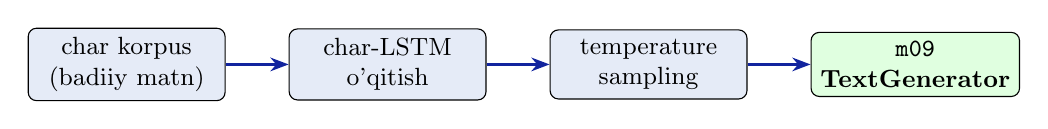
\begin{tikzpicture}[
      mod/.style={draw, fill=cnubluebg, rounded corners=3pt,
                  minimum width=2.5cm, minimum height=0.75cm,
                  font=\small, align=center},
      fin/.style={draw, fill=green!12, rounded corners=3pt,
                  minimum width=2.6cm, minimum height=0.75cm,
                  font=\small\bfseries, align=center},
      arr/.style={-{Stealth}, thick, color=cnublue}
  ]
    \node[mod] (co) {char korpus\\ (badiiy matn)};
    \node[mod, right=0.8cm of co]  (ls) {char-LSTM\\ o'qitish};
    \node[mod, right=0.8cm of ls]  (te) {temperature\\ sampling};
    \node[fin, right=0.8cm of te]  (m9) {\texttt{m09}\\ TextGenerator};
    \draw[arr] (co)--(ls); \draw[arr] (ls)--(te); \draw[arr] (te)--(m9);
  \end{tikzpicture}
  \end{center}
  \vspace{5pt}
  \begin{columns}[T]
    \begin{column}{0.50\textwidth}
      \textbf{P9 da qurasiz:}\\[3pt]
      \small
      \begin{itemize}\setlength\itemsep{2pt}
        \item \texttt{m09 TextGenerator}: char-LSTM \texttt{train}/\texttt{generate}
        \item Temperature bilan generatsiya ($0.3$/$0.7$/$1.2$)
        \item Temperature softmax $p(\text{nlp})$ ni tekshirish
      \end{itemize}
    \end{column}
    \begin{column}{0.46\textwidth}
      \textbf{Birinchi assert (bu slayd [I2]):}\\[4pt]
      \small\ttfamily
      assert abs(p\_nlp\_T1\\
      \phantom{xx}- 0.665) < 1e-3\\[4pt]
      \normalfont\footnotesize\color{halfgray}
      \textit{\# Ma'ruza L9 [I2]-slayd bilan}\\
      \textit{\# solishtiring (temperature)}
    \end{column}
  \end{columns}
\end{frame}

% ----------------------------------------------------------------
% [R] ADABIYOTLAR
% ----------------------------------------------------------------
\begin{frame}{Adabiyotlar}
  \begin{enumerate}\small\setlength\itemsep{5pt}
    \item Cho, K., van Merri\"enboer, B., va boshq.\ (2014). \textit{Learning Phrase
          Representations using RNN Encoder--Decoder...} EMNLP 2014.
    \item Graves, A.\ (2013). \textit{Generating Sequences With Recurrent Neural
          Networks.} arXiv:1308.0850. (Matn generatsiya, sampling.)
    \item Pascanu, R., Mikolov, T., Bengio, Y.\ (2013). \textit{On the difficulty of
          training RNNs.} ICML. (Gradient clipping.)
    \item Schuster, M., Paliwal, K.\ (1997). \textit{Bidirectional Recurrent Neural
          Networks.} IEEE Trans. Signal Processing.
    \item \texttt{torch.nn.LSTM(bidirectional=True)} / \texttt{clip\_grad\_norm\_} hujjatlari.
  \end{enumerate}
\end{frame}

% ================================================================
% [S] ILOVALAR (appendix --- slayd soniga kirmaydi)
% ================================================================
\appendix

\begin{frame}{Ilova S1: top-$k$ va top-$p$ (nucleus) sampling}
  \small
  Temperature --- yagona yo'l emas. Boshqa keng tarqalgan strategiyalar:
  \begin{itemize}\setlength\itemsep{2pt}
    \item \textbf{top-$k$}: faqat eng yuqori $k$ ta so'z orasidan tanlaymiz (qolganlari $0$).
    \item \textbf{top-$p$ (nucleus)}: yig'indi ehtimoli $p$ ga yetguncha eng yuqori
          so'zlarni olamiz.
  \end{itemize}
  \bunda{ikkalasi ham ``dumi uzun'' kam ehtimolli so'zlarni kesib, ma'nosiz tanlovlarni
  kamaytiradi; temperature bilan birga ishlatiladi.}
\end{frame}

\begin{frame}{Ilova S2: temperature chegaralarini keltirib chiqarish}
  \small
  $T\to 0^{+}$: eng katta $z_i$ uchun $e^{z_i/T}$ boshqalardan beqiyos katta bo'ladi
  $\Rightarrow p\to$ one-hot (argmax).
  $$ \lim_{T\to 0^{+}} \frac{e^{z_i/T}}{\sum_j e^{z_j/T}}
     = \begin{cases} 1 & z_i = \max_j z_j\\ 0 & \text{aks holda}\end{cases} $$
  $T\to\infty$: $z_i/T\to 0$ barcha $i$ uchun $\Rightarrow e^{0}=1 \Rightarrow$ bir tekis
  $p_i = 1/|V|$.
  \bunda{shuning uchun $T$ greedy ($T{=}0$) va tasodifiy ($T{=}\infty$) orasidagi silliq
  o'tish.}
\end{frame}

\end{document}
